\section{结论与展望}
你做到了! 我们已经到达终点线了。 在最后一章中,我们将简要回顾您通过本书实现的学习目标。 
我们不会得出结论,而是提出我们对大规模并行计算的未来的愿景,以及它的进步将如何影响未来的科学技术进程。

\subsection{重新审视目标}
正如我们在简介中所述,我们的主要目标是教读者如何对大规模并行处理器进行编程。 
我们承诺,一旦你培养出正确的直觉并以正确的方式去做,事情就会变得容易。 
特别是,我们承诺专注于计算思维技能,使您能够以适合并行计算的方式思考问题。 
我们还承诺将重点关注限制并行应用程序性能的因素,并提供系统的方法来优化代码以克服这些因素。

我们通过四个步骤兑现了这些承诺。 在第一步中,第 2 章到第 6 章介绍了并行计算和 CUDA C 的基本概念,
以及在 CUDA 中开发大规模并行代码时的关键性能考虑因素。 
他们还介绍了理解高性能并行编程中必须解决的硬件限制所需的相关计算机体系结构概念。 
有了这些知识,开发人员就可以自信地编写并行代码,并推理替代线程安排、循环结构和编码风格的相对优点。 
我们以常见优化技术清单来结束这一部分,我们在本书的其余部分中应用这些技术来优化各种并行模式和应用程序的性能。

在第二步中,我们介绍六种主要的并行模式(第 7 章到第 12 章),这些模式已被证明在将并行性引入许多应用程序中很有用。 
这些章节涵盖了最有用的并行计算模式背后的概念。 每个模式都用具体的代码示例进行说明。 
每个模式还用于介绍克服并行编程中经常遇到的并行化和性能障碍的重要技术。 
我们还使用这些模式来展示如何将第一步中引入的优化应用于各种场景。

第三步,我们介绍额外的高级模式和应用(第 13-19 章),以强化上一步中获得的知识和技能。 
虽然在这一步中,我们继续应用上一步中实践的优化,但我们更注重探索问题分解的替代形式,
以实现并行化并分析不同分解及其相关数据结构之间的权衡。 
这一步的最后一章致力于回顾计算思维技能(第 19 章,并行编程和计算思维),
帮助读者将前面几章中学到的概念概括为解决新问题所需的高级思维。 
有了这些见解,高性能并行编程就成为一种思维过程,而不是一种黑魔法。

第四步是让读者了解并行编程的相关高级实践。 
第 20 章“异构计算集群编程”介绍了使用 MPI 和 CUDA C 编程 HPC 集群所需的基本技能。
第 21 章“CUDA 动态并行性”介绍了动态并行性,可帮助并行程序员动态地解决更复杂的并行算法。 
许多实际应用程序中的工作负载各不相同。 
第 22 章,高级实践和未来演进,总结了其他高级实践以及对大规模并行处理器未来演进的期望。

我们希望您喜欢这本书,并同意我们的观点,即您现在已经做好了大规模并行计算系统编程的准备。

\subsection{未来展望}
\begin{figure}[H]
	\centering
	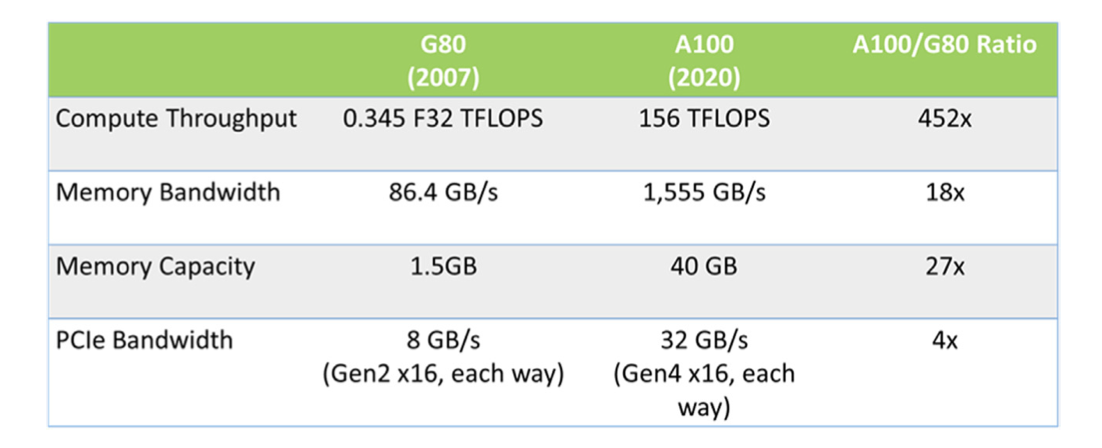
\includegraphics[width=0.9\textwidth]{figs/F23.1.png}
	\caption{\textit{从G80到A100,13年的对比。}}
\end{figure}

自 2007 年推出第一款支持 CUDA 的 GPU G80 以来,GPU 作为大规模计算设备的能力得到了惊人的提升,
计算吞吐量达到了 $452\times$ ,内存带宽达到了 $18\times$ ,如图 23.1 所示。 
这些进步刺激了科学和工程领域的高性能计算、人工智能和数据分析方面的巨大进步,
对金融、制造和医学等许多垂直领域产生了重大影响。 
例如,正如我们在第 16 章“深度学习”中看到的,GPU 引发了一场基于超大型数据集的深度学习革命,
并应用于图像识别、语音识别和视频分析。

自 2010 年本书第一版以来,并行计算领域也以惊人的速度发展。 可使用可扩展算法解决的问题范围已显着扩大。 
虽然 GPU 的使用最初集中于常规密集矩阵计算和蒙特卡罗方法,但其用途已迅速扩展到稀疏方法、图计算和自适应细化方法。 
在许多领域,算法也取得了快速进步。 并行模式、高级模式和应用章节中介绍的一些算法代表了最新的重大进展。

我们中的一些人很自然地想知道并行计算的快速发展是否已到达终点。 从种种迹象来看,答案肯定是否定的。 
我们正处于并行计算革命的开始阶段。 过去三十年计算技术取得的惊人进步引发了行业的范式转变。 
过去,重大创新是由计算设备辅助的物理仪器驱动的。 它们现在由物理仪器辅助的计算驱动。

例如,二十年前,GPS 彻底改变了我们的驾驶方式。 GPS 主要基于卫星信号感测,并辅以计算方法来确定两个位置之间的最短路径。 
最近,通过手机中的地图应用程序和云中的数据服务进行的同行报告和计算进一步使驾驶员能够根据交通状况改变路线。 
如今,汽车行业最激动人心的革命是自动驾驶汽车,它主要基于物理传感器辅助的机器学习计算方法。

再比如,MRI和PET在过去二十年里彻底改变了医学。 这些技术主要基于电磁和光传感器,并辅以计算图像重建方法。 
他们允许医生在不进行手术的情况下观察人体内部的病理情况。 
如今,医学领域正在经历个体化医疗革命,这场革命主要是由测序传感器辅助的计算基因组学方法驱动的。

再举一个例子,半导体行业过去依赖于物理光源的进步,并辅以计算方法,这些计算方法强制执行设计规则,
以减少制造过程中的设备特征尺寸。 如今,物理光源的进步实际上已经停止。 
特征尺寸减小的进步主要是由光刻掩模驱动的,光刻掩模经过计算设计,可以协调光波的干扰,从而在芯片上产生极其精确的蚀刻图案。

许多其他领域也发生了同样的范式转变。 计算已成为我们社会中几乎所有令人兴奋的创新的主要驱动力。 
这对更快的计算系统产生了无法满足的需求。 正如我们在第一章简介中讨论的那样,并行计算是提高计算性能的唯一可行方法。 
这种强大的需求将继续激励业界创新并创造更强大的并行计算设备。 
最有潜力改进的领域之一是访问存储数据的并行性级别,过去这是通过非常低的并行性级别完成的。 
访问海量存储数据的根本性改进可能会激发我们目前无法想象的整整一代应用程序。

总之,我们正处于计算黄金时代的黎明。 业界将继续招募和奖励高技能的并行程序员。 
您的工作将为您选择的领域带来真正的改变。

享受这一旅程!